\chapter{Being Hurt and Hurting Others}

This chapter follows J. Krishnamurti's dialogue with Dr. Alan W. Anderson on religion, attention, hurt, and education, in source material credited to J. Krishnamurti and the Krishnamurti Foundation Trust, with curation by LazyingArt LLC. There are no validated blackboard frames for this lecture, so the displayed mathematics below is not a claim about equations on a board. It is a compact notation for the order of the inquiry. The source remains the spoken movement: thought is not to be abolished; rather, we ask what thought can do, what it cannot do, what attention is, and why psychological hurt prevents a mind from being whole.

\section{Religion Before Belief}

Anderson begins by correcting a possible misunderstanding. In the earlier conversations, Krishnamurti has not said that thought should be destroyed. He has not said that knowledge, as such, is diseased. The difficulty is more exact: thought and knowledge become dysfunctional when they try to occupy the place of intelligence, relationship, and the immeasurable.

That question leads Anderson to religion. Perhaps the human idea of God arose from some relation to an abiding activity; perhaps that idea has then been abused. Krishnamurti does not begin by accepting the inherited word. He first clears the ground. Words such as religion, love, and God have been so abused that they have almost lost their meaning. Religion, as ordinarily practiced, has become superstition, propaganda, belief, ritual, and the worship of images made by hand or by mind.

A compact way to mark the rejected map is:
\begin{equation}
\text{religion}_{\text{common}}
\Rightarrow
\text{belief}+\text{ritual}+\text{fear}+\text{image}+\text{authority}.
\end{equation}
This is not Krishnamurti's definition. It is the structure he is refusing. The word has become tied to systems of consolation and belonging, and therefore to thought's search for security.

The correction is deliberately simple:
\begin{equation}
\text{religion}_{\text{inquiry}}
\Rightarrow
\text{gathering of total energy}.
\end{equation}
Religion, in the sense used here, is not a system of belief about an object called God. It is the gathering of energy at all levels--physical, moral, and spiritual--so that there is attention.

\subsection{Question \& Answer}

\paragraph{Question.}
If thought is not to be abolished, why can thought not be the instrument that reaches the religious or the immeasurable?

\paragraph{Answer.}
Because in this dialogue thought is described as conditioned, fragmentary, never new, and never free. Thought has its necessary place, but it cannot capture what is beyond its own measure. The task is not to attack thought, but to see its limit.

\begin{equation}
\text{thought}
\Rightarrow
\text{conditioned}+\text{fragmentary}+\text{not new}+\text{not free}.
\end{equation}

This gives the lecture its first real tension. If thought is limited, and if religion is not belief, then what kind of movement can meet what thought cannot capture?

\section{Gathering Energy Into Attention}

Krishnamurti's answer is attention. Religion means the gathering together of energy, and that gathering brings about great attention. In that attention, he says, there is no frontier. This is the axis of the first half of the conversation.

We should not make this into an inward exercise with a reward at the end. He is not recommending concentration, breath control, or a program of spiritual attainment. He is distinguishing the mechanical action of thought from the quality of attention in which thought is understood.

\begin{definition}
In this chapter, \emph{attention} means the gathering of the whole energy of the human being--brain, mind, heart, nerves, and perception--without exclusion, resistance, effort, frontier, or expectation.
\end{definition}

The spoken structure may be written schematically as:
\begin{align}
\text{gathering of energy}
&\Rightarrow \text{attention},\\
\text{attention without frontier}
&\Rightarrow \text{perception beyond the measure of thought}.
\end{align}

The word ``beyond'' must remain sober. Krishnamurti explicitly rejects romanticism, speculation, and sentimentality. Beyond thought does not mean vague belief. It means that thought, being conditioned and fragmentary, cannot possess the whole.

\begin{figure}
\centering
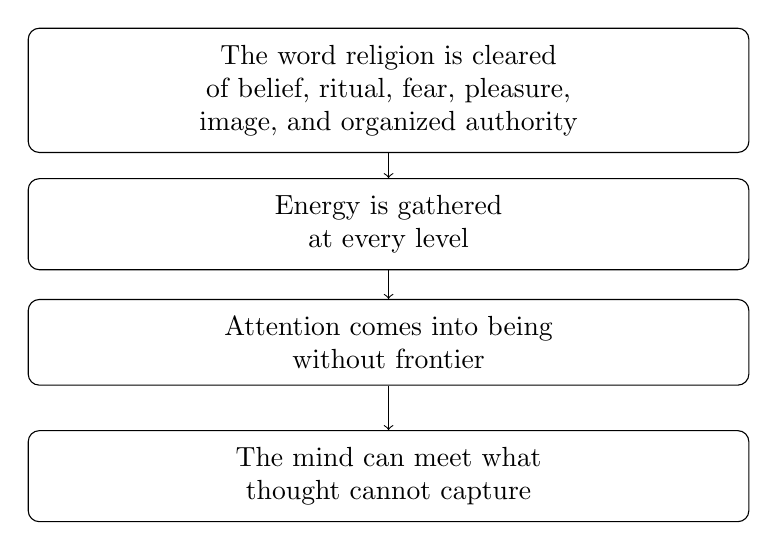
\begin{tikzpicture}
\node[draw, rounded corners, text width=.72\linewidth, align=center, inner sep=6pt] (a) at (0,0)
{The word religion is cleared\\of belief, ritual, fear, pleasure,\\image, and organized authority};
\node[draw, rounded corners, text width=.72\linewidth, align=center, inner sep=6pt] (b) at (0,-1.7)
{Energy is gathered\\at every level};
\node[draw, rounded corners, text width=.72\linewidth, align=center, inner sep=6pt] (c) at (0,-3.2)
{Attention comes into being\\without frontier};
\node[draw, rounded corners, text width=.72\linewidth, align=center, inner sep=6pt] (d) at (0,-4.9)
{The mind can meet what\\thought cannot capture};
\draw[->] (a) -- (b);
\draw[->] (b) -- (c);
\draw[->] (c) -- (d);
\end{tikzpicture}
\caption{A transcript-based reconstruction of the opening movement: religion is redefined as gathered energy becoming attention.}
\end{figure}

The diagram is an analytic reconstruction, not a blackboard reproduction. Its purpose is to preserve the order of the lecture: first clear the word, then gather energy, then understand attention, then ask what thought cannot capture.

\section{The Priest, Fear, and the Loss of Nature}

Anderson responds by bringing in biblical language: stillness, the inadequacy of human thought, and the difference between human ways and divine ways. Krishnamurti shifts the scale. He does not stay with scripture as authority. He turns to what happens when human beings lose direct contact with nature--with clouds, lakes, birds, the earth, and the beauty of seeing.

When that contact is lost, the priest enters. The priest becomes mediator between the human being and the so-called divine. He interprets, explains, commands, and exploits. What was simple becomes mixed up. What was direct becomes mediated. What was adoration of beauty becomes fear and propaganda.

The structure is important enough to write down:
\begin{equation}
\text{loss of contact with nature}
\Rightarrow
\text{mediation}
\Rightarrow
\text{authority}
\Rightarrow
\text{fear}.
\end{equation}

This is not merely a historical complaint. It explains why religion becomes one of the false maps of happiness. The priest offers something beyond the daily round of bread, house, work, desire, and death. He appears to offer security, grace, continuity, and preservation. But the security is purchased through fear.

Krishnamurti then returns to the earlier definition. If religion is the gathering of energy into total attention, organized fear is not religion. The measurable and mechanical have their place, but when life becomes merely mechanical, another reaction appears: superstition, gurus, rituals, and promises of spiritual safety. The measurable breeds its opposite when it becomes the whole of life.

\section{The Religious Mind and the Quiet Mind}

The lecture now moves from institutions to the quality of mind. Krishnamurti asks what kind of mind can perceive something beyond the measurement of thought. He repeats the question because it is not rhetorical. It is the engine of the middle movement.

A mind that can perceive must be quiet. This quietness is not induced silence, withdrawal, obedience, or discipline imposed by will. It is a simple fact: if the mind is chattering, it does not listen. If it is occupied with itself, it cannot attend.

\begin{proposition}
Within this dialogue, quietness is not a decorative spiritual state; it is a condition of direct perception.
\end{proposition}

\begin{proof}
Perception requires listening and seeing. A mind occupied with its own movement does not listen or see directly. The chattering movement of thought occupies the mind with itself. Therefore, for perception to be direct, the mind must be quiet. This is not a method for becoming quiet; it is the recognition that in psychological noise, attention is absent.
\end{proof}

Anderson then tests the language of devotion and one-pointedness. Krishnamurti immediately asks whether attention is one-pointed. The question matters because one-pointedness can easily become focus, and focus can become exclusion.

\subsection{Question \& Answer}

\paragraph{Question.}
Is attention one-pointed?

\paragraph{Answer.}
Not if one-pointedness means concentration on an object. Anderson clarifies that he means integrated rather than focused, but Krishnamurti's question exposes the danger. If attention is made into a point, it may become concentration; and concentration, in this dialogue, excludes.

\begin{table}
\centering
\begin{tabular}{|p{.42\linewidth}|p{.42\linewidth}|}
\hline
\textbf{Concentration} & \textbf{Attention} \\
\hline
Brings thought to a point & Gives the whole energy of being \\
\hline
Excludes what is not selected & Does not exclude \\
\hline
Builds a barrier around focus & Has no frontier \\
\hline
Involves effort and resistance & Has no resistance and no effort \\
\hline
Can strengthen division & Sees division and duality \\
\hline
\end{tabular}
\caption{A transcript-based contrast between concentration and attention.}
\end{table}

The same test is applied to receptivity and waiting. If we say the mind is receptive, Krishnamurti asks who is there to receive. If we say the mind waits, then there is one who waits and something expected. Again duality has entered. The lecture proceeds by removing these subtle divisions.

\begin{equation}
\text{waiting}
\Rightarrow
\text{one who waits}+\text{something expected}.
\end{equation}

So the inquiry holds to the word attention. Attention is not concentration, not reception, not expectation, and not a refined form of waiting. It is the total energy of perception without a center seeking a result.

\section{Why Human Beings Are Hurt}

At this point Krishnamurti gathers the earlier themes. A mind that is attentive has understood relationship and responsibility, has understood psychological fear, and has understood the movement of pleasure. Then comes the next question: what is such a mind? The answer is not abstract. It requires looking at hurt.

He distinguishes physical pain from psychological hurt. Physical pain can be watched; it need not corrode the whole quality of mind. Psychological hurt is more difficult because it enters the structure of the self. A hurt mind is not innocent, and this lack of innocence prevents total attention.

\begin{definition}
\emph{Psychological hurt}, in this chapter, means the wound sustained by the image one has of oneself. It is distinct from physical pain, and it is not merely the thought that one has been hurt.
\end{definition}

The transcript contains an uncertain etymological phrase around the word innocence. We should not build an etymology on that uncertainty. The conceptual point is clear enough: Krishnamurti is using innocence to mean a mind not hurt, or a mind incapable of being hurt.

Anderson proposes that hurt may arise when one starts thinking about thinking that one is hurt. Krishnamurti says the matter is deeper. From childhood, the child is compared with another child. That comparison is already the beginning of hurt.

\begin{align}
\text{comparison}
&\Rightarrow \text{image of oneself},\\
\text{image of oneself}
&\Rightarrow \text{resistance wall},\\
\text{wall touched at a tender point}
&\Rightarrow \text{hurt}.
\end{align}

This is not a formal law. It is a disciplined shorthand for the movement Krishnamurti describes. The image is a wall between you and me. When that wall is touched at its tender point, I am hurt.

\subsection{Question \& Answer}

\paragraph{Question.}
Is hurt simply a matter of thinking about the fact that one has been hurt?

\paragraph{Answer.}
No. The lecture says the matter is deeper. Hurt begins with comparison, imitation, and the building of an image. Thought may sustain and repeat the hurt, but the vulnerable structure is the image itself.

\paragraph{Worked example.}
Suppose a child is told, ``Your brother is clever; you are not.'' The sequence is not merely that the child hears a sentence. The sentence introduces comparison. Comparison invites an image: ``I am the inferior one.'' That image becomes a point of resistance. Later, another casual word touches the same image, and the hurt repeats.

\begin{equation}
\text{comparison: ``he is clever, I am not''}
\Rightarrow
\text{self-image}
\Rightarrow
\text{woundable identity}.
\end{equation}

The same structure appears with name, body, class, status, nationality, family, and tradition. A name by itself is not the problem. ``Mr. Brown'' is only a name. The problem begins when thought builds an image around the name: superior, inferior, ancient family, respectable class, Brahmin, non-Brahmin, aristocrat, success, failure.

\begin{equation}
\text{name}+\text{body}+\text{status}+\text{tradition}+\text{propaganda}
\Rightarrow
\text{image sustained by thought}.
\end{equation}

Krishnamurti's point about the word and the thing enters here. If one sees that the word is not the thing and the description is not the described, then the sacredness of a name, even the name of God, loses its psychological power. The danger is not sound or spelling; it is identification.

\section{Healing Hurt Without Making a Method}

The lecture then raises two questions with unusual clarity. Can the hurts already received be healed so that not a mark is left? And can future hurt be prevented completely, without resistance, withdrawal, or escape? The transcript is slightly garbled at this point, but the intended contrast is clear: no more hurt does not mean building a defensive wall.

These are two sides of one inquiry:
\begin{align}
Q_1 &: \text{Can past hurt end without leaving a mark?}\\
Q_2 &: \text{Can future hurt not be added?}
\end{align}
The labels \(Q_1\) and \(Q_2\) are only a shorthand for the spoken questions.

Anderson suggests that complete attention might dissolve the image. Krishnamurti agrees only after making a crucial correction. We cannot use attention as a means to wipe away hurt. That would turn attention into a method, and method belongs to the old mechanical movement.

\subsection{Question \& Answer}

\paragraph{Question.}
Can attention be used as a tool to wipe away hurt?

\paragraph{Answer.}
No. The order is the reverse. One must understand the image, hurt, education, family, and society in which the image was formed. Out of that understanding comes attention. If I am hurt and simply try to apply attention as a remedy, I am still acting from hurt.

\begin{equation}
\text{understanding hurt}
\Rightarrow
\text{attention},
\qquad
\text{not}
\qquad
\text{attention as technique}
\Rightarrow
\text{erasure of hurt}.
\end{equation}

This is one of the safeguards of the chapter. The inquiry must not become a program. Krishnamurti asks us to look at hurt, not translate it, not wish to wipe it away, not escape it, but see it. The seeing includes insults, negligence, casual words, gestures, and the language that wounds.

From hurt, a series of reactions follows:
\begin{equation}
\text{hurt}
\Rightarrow
\text{violence}+\text{fear}+\text{withdrawal}+\text{search for safety}.
\end{equation}
The search for safety may even create an idea of God as one who will never hurt. Here the beginning of the lecture returns: religion made by fear is not religion; it is a projection of hurt.

\section{Education as the Act of Love}

The last movement translates the inquiry into education. Anderson raises the case of a child who arrives at school already hurt. Krishnamurti says that the child is already hurt, and hurt because it is hurt. From hurt come violence, fear, withdrawal, neurotic action, and the acceptance of anything that promises safety.

The ordinary response is to continue the very structure that produced the hurt. The parent compares. The school gives marks. The teacher transmits information. Society praises imitation. Even religion says, ``Be like Krishna, Buddha, or Jesus.'' Krishnamurti says this too is hurt.

\begin{equation}
\text{comparison}+\text{imitation}+\text{ideal}
\Rightarrow
\text{hurt sustained by culture}.
\end{equation}

The educational problem is therefore not secondary. It is the concrete test of the inquiry:
\begin{equation}
\text{hurt parent}+\text{hurt teacher}+\text{hurt child}
\Rightarrow
\text{civilization continues hurt}.
\end{equation}

But another relation is possible. When the educator realizes that he is hurt and that the child is hurt, the relationship changes. In the very act of teaching--whether the subject is mathematics or anything else--he is freeing himself from hurt and helping the child be free of hurt.

\begin{figure}
\centering
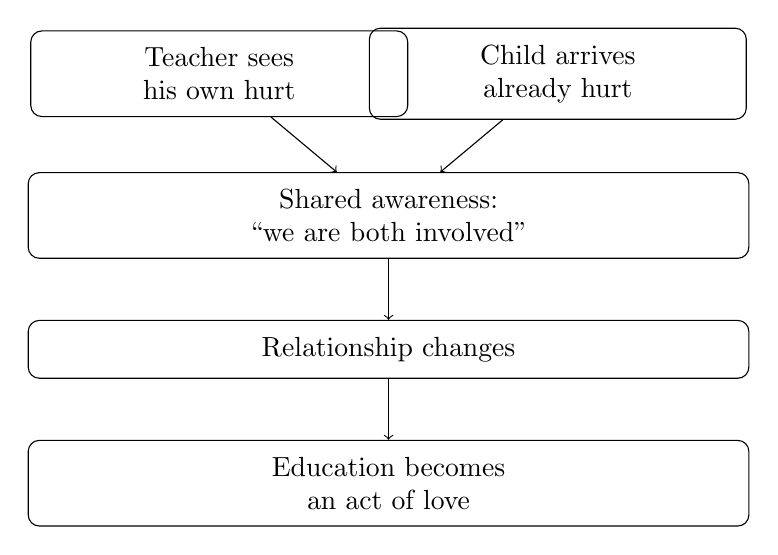
\begin{tikzpicture}
\node[draw, rounded corners, text width=.36\linewidth, align=center, inner sep=6pt] (t) at (-2.15,0)
{Teacher sees\\his own hurt};
\node[draw, rounded corners, text width=.36\linewidth, align=center, inner sep=6pt] (c) at (2.15,0)
{Child arrives\\already hurt};
\node[draw, rounded corners, text width=.72\linewidth, align=center, inner sep=6pt] (s) at (0,-1.8)
{Shared awareness:\\``we are both involved''};
\node[draw, rounded corners, text width=.72\linewidth, align=center, inner sep=6pt] (r) at (0,-3.5)
{Relationship changes};
\node[draw, rounded corners, text width=.72\linewidth, align=center, inner sep=6pt] (l) at (0,-5.2)
{Education becomes\\an act of love};
\draw[->] (t) -- (s);
\draw[->] (c) -- (s);
\draw[->] (s) -- (r);
\draw[->] (r) -- (l);
\end{tikzpicture}
\caption{A transcript-based reconstruction of the educational relation: hurt is not solved by information, but by shared seeing in relationship.}
\end{figure}

The teacher does not begin with a subject alone. He begins by seeing what hurt does: it kills, destroys, produces violence, and makes one want to hurt others. Only then can teaching become relationship rather than transmission.

Anderson then asks a subtle question. If a student is hurt-bound, will he not misinterpret the action of one who is not hurt-bound? Krishnamurti's answer is stark: there are very few who are not hurt-bound. He says, humbly but directly, that many things have happened to him, and yet he does not know what it means to be hurt. Whether or not the reader can say this, the educational demand remains: it is possible not to add hurt.

At the end Anderson asks whether they might next take up the relationship of love to all this. Krishnamurti agrees. The chapter closes there because the word love has now been prepared. It is not sentiment, coercion, or a reward for correct behavior. In this lecture it first appears as the act in which teacher and child see hurt together and help each other be free of it.

\section{Summary}

The chapter has one continuous movement. Thought is not denied, but its limit is seen. Religion is not belief, ritual, or authority; in this inquiry it is the gathering of total energy into attention. Attention is not concentration, receptivity, waiting, or method. It has no exclusion, resistance, effort, or frontier.

The obstacle to such attention is psychological hurt. Hurt is not merely the idea that one has been hurt; it is rooted in comparison, imitation, self-image, name, status, and identification. The image becomes a wall, and when the wall is touched, the person is wounded.

The final movement is educational and relational. Can past hurt end without leaving a mark, and can future hurt not be added? The answer is not a technique. It begins in understanding hurt directly. In education, that means the teacher and child see together that both are hurt. When that seeing changes relationship, Krishnamurti calls it an act of love.